\documentclass[10pt, a4paper]{article}
\usepackage[latin1]{inputenc}
\usepackage{graphicx}
\usepackage[pdftex, linkbordercolor={0 0 1}]{hyperref}
\usepackage{float}
\usepackage{amsfonts}
\usepackage{lscape}
\parindent0pt

\graphicspath{{images/}}

\newcommand{\req}[1]{\textsuperscript{(req. \ref{#1})}}
\newcommand{\reqdefLabel}[1]{\label{#1}}
\newcommand{\reqdef}[1]{\textbf{(see \ref{#1})}}
\newcommand{\saf}[1]{\emph{see also Figure \ref{fig: #1}}}

\begin{document}
\title{MiXiM - Physical Layer}
\author{Karl Wessel: wessel$@$tkn.tu-berlin.de\\
Michael Swigulski: swigulski$@$tkn.tu-berlin.de}
\date{20. November 2007}
\maketitle
%\section{Preamble}

\subsection{What is the Physical Layer}
TODO: write description

\section{requirement specification}
\label{req_spec}

\subsection{Overview}
\label{overview}

\begin{itemize}
 \item provide status information to MAC
 \item switch radiostate (RX, TX, SLEEP)
 \item send packets to air/channel
 \item receive packets / listen for packets
 \item provide hooks for statistical information
 \item configurable settings
\end{itemize}

\subsection{provide status information to MAC}
\label{stateInfo}

In addition to received packets the physical layer has to provide some other information to the MAC layer.
Some of this information has to be provided passively\reqdefLabel{defprovpassive} on demand (e.g. current channelstate) and some should be delivered actively\reqdefLabel{defprovactive} to the MAC layer on certain events (e.g. transmission of a packet complete).

\noindent Information which has to be provided to MAC on demand:
\begin{itemize}
 \item channelstate: busy/idle (boolean) or RSSI\reqdefLabel{defchannelstate}
 \item current radiostate (RX, TX, SLEEP)\reqdefLabel{defcurrentmode}
\end{itemize}

\noindent Information which has to be provided to MAC the moment it occurs:
\begin{itemize}
 \item transmission over (send)\reqdefLabel{deftxover}
\end{itemize}


\subsection{switch radiostate}
\label{switchstates}

The physical layer has to be able to switch between the following things:

\begin{itemize}
 \item current radiostate (RX, TX, SLEEP)\reqdefLabel{defswitchmode}
\end{itemize}

Switching from one state to another may take some time. Whereas the switching time may depends to whitch state we are switching.\reqdefLabel{defswitchtimes}

\begin{figure}[H]
 \centering
 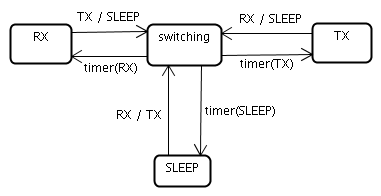
\includegraphics[width=240pt]{req_spec/stateMachineMode.png}
 % stateMachineMode.png: 1179666x1179666 pixel, 0dpi, infxinf cm, bb=
 \caption{State machine for radiostate}
 \label{fig: mode state machine}
\end{figure}


\subsection{send packets}
\label{subSendPackets}

The physical layer has to be able to send packets from the MAC layer to the channel. 
We also want to support the possibility to control
the sending process after it has been started.\reqdefLabel{defsendControl}

Before we can send packets the following things have to be 
assured:
% \linebreak
\begin{itemize}
 \item the radio has to be in TX state\reqdefLabel{defsendPreqMode}
 \item we are not already sending\reqdefLabel{defsendPreqSending}
% \item the channel should be idle (this is no hard requirement)\reqdefLabel{defsendPreqIdle}
\end{itemize}

The above items should be controlled by the MAC layer so the physical layer would only throw an error if they are not set.

The following information has to be attached by the MAC layer to the packet:

\begin{itemize}

 %\item channel\reqdefLabel{defsendCtrlChannel}
 \item channel dimensions (frequency/space)\reqdefLabel{defsendCtrlChannel}
 %\item header bitrate\reqdefLabel{defsendCtrlHeaderBitrate}
 %\item payload bitrate\reqdefLabel{defsendCtrlBitrate}
 \item bitrate (for all dimensions) over time\reqdefLabel{defsendCtrlHeaderBitrate}\reqdefLabel{defsendCtrlBitrate}\\
 \emph{Note: Most cases will be covered by header and payload bitrate.}
 \item TX power for all dimensions over time\reqdefLabel{defsendCtrlTXPower}
 
 \item size of packet\reqdefLabel{defsendCtrlSize}
\end{itemize}


The sending process itself is made up of the following steps:

\begin{enumerate}\reqdefLabel{defpacketFromMac}\reqdefLabel{defsendInfoTXPower}\reqdefLabel{deftxover2}\reqdefLabel{defsendToChannel}
 \item MAC layer gives packet and control info to physical layer
 \item check requirements for sending, throw error if they are not fulfilled
 \item add information needed by the receiving physical layer to packet (see below)
 %\item add signal function (transmission power\footnote{The receiver converts the same signal to receiving power over time.} over time)\footnote{The signal function could be more dimensional. E.g.: receiving power over time and channel.} to packet
 \item add signal to packet
 \item packet is sent to channel by physical layer
 \item schedule transmission over message for MAC layer
\end{enumerate}

The following information is needed by the receiving physical layer:

\begin{itemize}
\item signal
	\begin{itemize}
	\item TX power (for all dimensions) over time
	\item the bitrate (for all dimensions) over time\reqdefLabel{defsendInfoBitrate} 
	\item the channel(dimensions)\reqdefLabel{defsendInfoChannel}
	\item the duration the signal would need to be transmitted\reqdefLabel		{defsendInfoDuration}
	\item the duration of the preamble\reqdefLabel{defsendInfoPreambleDuration}
	
	\end{itemize}
\item position, move direction and speed of the sending host\reqdefLabel{defsendInfoMove}
\item size of packet\reqdefLabel{defsendInfoSize}
\end{itemize}

\subsection{receive packets}
\label{receivePackets}

Because the packets arrive immediately at every receiving node we have to
simulate the receiving process:

\begin{enumerate}\reqdefLabel{defrcvSimDelay}\reqdefLabel{defrcvSimPreamble}\reqdefLabel{defrcvSimDuration}
\item simulate propagation delay (if needed)
\item simulate preamble duration
\item simulate payload duration
\end{enumerate}

We also have to simulate the attenuation of the signal strength\reqdefLabel{defrcvSimAttenuation}. This should be done by filtering the signal with the \textit{analogue models} directly after a message arrives (since we already have it then). The AnalogueModels will add an attenuation matrix to the Signal.\\

%If the preamble is transmitted the packet has to be classified as
\textit{signal} or \textit{noise}\reqdefLabel{defrcvClassify}. The decision is
made by the \textit{Decider}. Therefore the preamble has to be filtered
previously by the analogue models.\reqdefLabel{defrcvFilterPreamble}

The packet has to be classified as \textit{signal} or
\textit{noise}\reqdefLabel{defrcvClassify}. The decision is made by the
\textit{Decider}.\\

If the transmission of a \textit{signal} is over we have to decide if it was
received correctly.\reqdefLabel{defrcvIsCorrect} This is also done by the
\textit{Decider} by evaluating the \textit{signal to noise ratio} short
\textit{SNR}. 
If the signal was received correctly we pass it to the MAC
layer.\reqdefLabel{defrcvPassToMAC} It is also possible to pass the signal to
the MAC layer anyway, marked as biterror/collision.

\subsubsection{the analogue model}
\label{analogueModel}

The \textit{analogue model} simulates the attenuation of the signal strength by
filtering the receiving power function\reqdefLabel{defanalogueFilter}.

There should be models to simulate the following things:

\begin{itemize}
 \item pathloss\reqdefLabel{defanalogueSimPathloss}
 \item shadowing\reqdefLabel{defanalogueSimShadowing}
 \item fading\reqdefLabel{defanalogueSimFading}
\end{itemize}

Further we set the following requirements to the \textit{analogue models}:

\begin{itemize}
 \item physical layer should be able to apply multiple \textit{analogue models}
to a signal\reqdefLabel{defanalogueMulti}
 \item you should be able to set the \textit{analogue models} independent from
physical layer\reqdefLabel{defanalogueIndependent}
 \item you should be able to add your own \textit{analogue
models}\reqdefLabel{defanalogueExtensible}
\end{itemize}

\subsubsection{the Decider}
\label{Decider}

As mentioned already above the \textit{Decider} has to decide the following
things:

\begin{itemize}
\item classify packet as \textit{signal} or
\textit{noise}\reqdefLabel{defrcvClassify2}
\item decide if a packet was received correctly on the basis of the signal and 
interfering noise\reqdefLabel{defrcvIsCorrect2}
\end{itemize}

We set the following requirements to the \textit{Decider}:

\begin{itemize}
 \item you should be able to set the \textit{Decider} independently from
physical layer\reqdefLabel{defdeciderIndependent}
 \item you should be able to add your own
\textit{Decider}\reqdefLabel{defdeciderExtensible}
 \item the \textit{Decider} should be able to return bitwise correctness of the
\textit{signal} (on demand)\reqdefLabel{defdeciderBitwise}
\end{itemize}


\subsection{statistical information}
\label{statistic}

You should be able to get the following statistical information (the physical
layer should not evaluate it but has to provide access to the according
information):

\begin{itemize}
\item packet count\reqdefLabel{defstatPackets}
\item received signal strength\reqdefLabel{defstatRSS}
\item signal to noise ratio\reqdefLabel{defstatSNR}
\item bit error ratio\reqdefLabel{defstatBER}
\item collisions\reqdefLabel{defstatColls}
\end{itemize}

\subsection{parameters}
\label{parameters}

The following parameters of the physical layer should be freely configurable:

\begin{itemize}
	\item simulate propagation delay? (boolean)\reqdefLabel{defconfDelay}
	\item which analogue models should be used\reqdefLabel{defconfAnalogue}
	\item the parameters for the analogue models\reqdefLabel{defconfAnalogueParam}
	\item which Decider should be used\reqdefLabel{defconfDecider}
	\item the parameters for the decider\reqdefLabel{defconfDeciderParam}
	\item thermal noise\reqdefLabel{defconfNoise}
	\item sensitivity\reqdefLabel{defconfSens}
	\item maximum TX power\reqdefLabel{defconfMaxTXPower}
	\item switching times between states (RX, TX, SLEEP)\reqdefLabel{defconfSwitchingTimes}
\end{itemize}





%
















\newcommand{\h}[1]{\textit{#1}}
\newcommand{\bp}{BasePhyLayer}
\newcommand{\bm}{BaseMacLayer}


\section{modelling}


\subsection{overview}

Here we present the design- and interface details of the OMNeT-module 
\h{\bp}\footnote{We denote a Layer in a general meaning by 'physical layer' or
 'MAC layer' and our concrete C++ classes
by \h{\bp} or \h{\bm}.} to meet the requirement specification. That includes:

\begin{enumerate}
 \item internal class diagram of \h{\bp} and relation to \h{\bm}
 \item interface description for all involved C++ classes
 \item flow charts for reception of MacPacket from upper layer and 
 AirFrame from the channel
 \item some detailed flow charts for important sub processes
\end{enumerate}


\subsection{classgraph}

We start with the classgraph for the OMNeT-module \h{\bp} that shows its C++ classes,
 relations to other OMNeT-modules (especially \h{\bm})
and the OMNeT-messages sent between them.\\

The \h{\bp} holds a list\req{defanalogueMulti} of AnalogueModels and a pointer
to a
Decider. Thus the AnalogueModel and the Decider are submodules of \h{\bp}. This
way one is able to change\req{defanalogueExtensible}\req{defdeciderExtensible}
and
replace\req{defanalogueIndependent}\req{defdeciderIndependent} them
independently from
the \h{\bp}.

\begin{landscape}
\begin{figure}
 \centering
 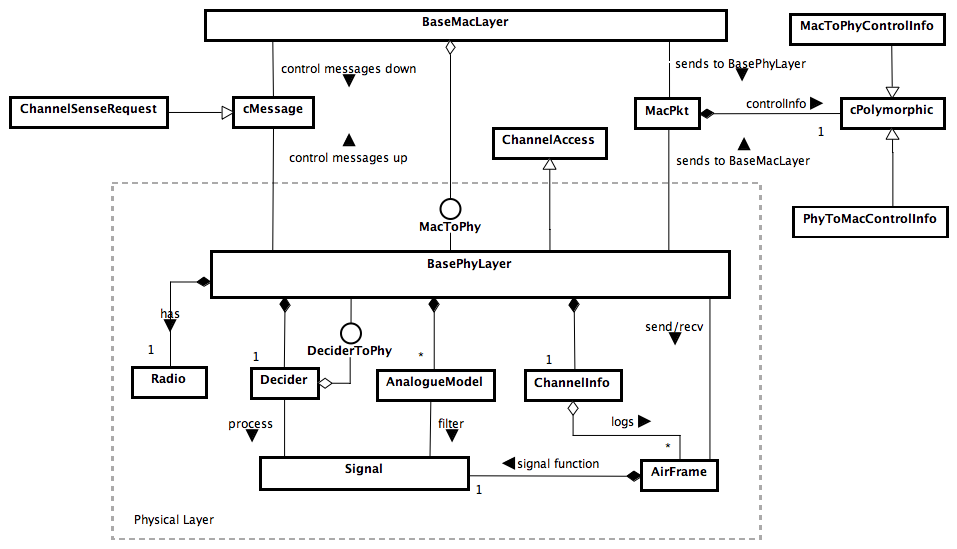
\includegraphics[width=21cm]{modelling/class_diagram.png}
 \caption{class graph}
 \label{fig: classgraph}
\end{figure}
\end{landscape} 

\subsection{The \bp}

In this section we focus on the module \h{\bp} and how one is able to communicate with the 
it, i.e. especially the \h{\bm} which is connected to the \h{\bp}
in three ways:

\begin{enumerate}
 \item OMNeT-channel for data messages
 \item OMNeT-channel for control messages
 \item a reference to the \h{MacToPhyInterface}.
\end{enumerate} 

The \underline{data channel} is used to send and receive\req{defpacketFromMac}
MacPkts to and
from the \h{\bp}. An appropriate ControlInfo is attached to the packet by the
sending layer. The \h{MacToPhyControlInfo} is the carrier of the Signal from the
MAC-Layer down to the Physical-Layer.
\saf{MacToPhyCtrlInfo interface}\\

The \underline{control channel} is used by the \h{\bp} to inform the \h{\bm}
about
certain events\req{defprovactive}, e.g. the TX\_OVER\req{deftxover} message 
which indicates the end of a sending transmission.

A ChannelSenseRequest can be sent over \underline{control channel} from \h{\bm}
to \h{\bp}. It is handed to the Decider (several times) that attaches a
ChannelState and finally sent back to \h{\bm}.
\begin{figure}[H]
 \centering
 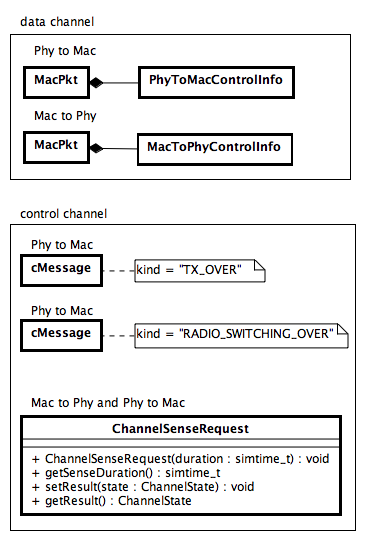
\includegraphics[width = 0.7\textwidth]{modelling/PhyMacMessages.png}
 \caption{messages sent between \h{\bp} an \h{\bm}}
 \label{fig: PhyMacMessages}
\end{figure}


The \underline{reference} provides a passive way\req{defprovpassive} for the  \h{\bm} to 
get
information about the current channel state\req{defchannelstate} (that is an
alternative [immediate answer] to sending a ChannelSenseRequest) and to
get\req{defcurrentmode} and set\req{defswitchmode} the current radiostate (RX,
TX,
SLEEP).
Switching times\req{defswitchtimes} from one radio state to another are
controlled
internally by a state machine. \saf{mode state machine} and \ref{radio}
\\
This functionality offered to \h{\bm} beside OMNeT is defined by the \h{MacToPhyInterface}.
\\

Further the \h{\bp} has an interface \h{DeciderToPhyInterface} that defines the functionality
needed by the Decider. (see also \ref{decider})
% interface description here
\label{SignalCreation}

\begin{figure}[H]
 \centering
 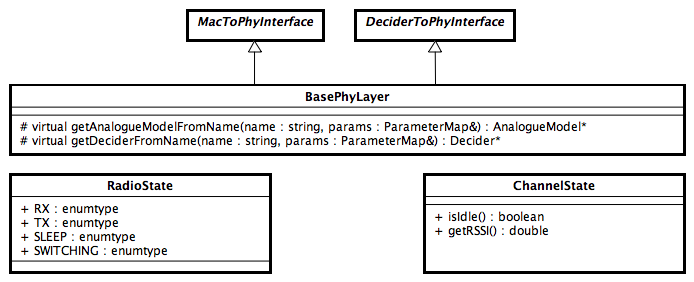
\includegraphics[width = \textwidth]{modelling/BasePhyLayer_members.png}
 \caption{BasePhyLayer interface}
 \label{fig: BasePhyLayer interface}
\end{figure}

\begin{figure}[H]
 \centering
 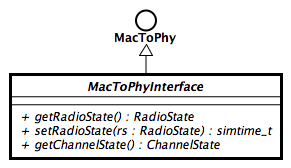
\includegraphics{modelling/MacToPhyInterface_members.png}
 \caption{MacToPhy interface}
 \label{fig: The MacToPhyInterface}
\end{figure}

\subsection{Radio}
\label{radio}

The Radio-class implements the radio of the host as a state machine under supervision
of the \h{\bp}. Instructions from \h{\bm} concerning the radio are handled by \h{\bp}.

\begin{figure}[H]
 \centering
 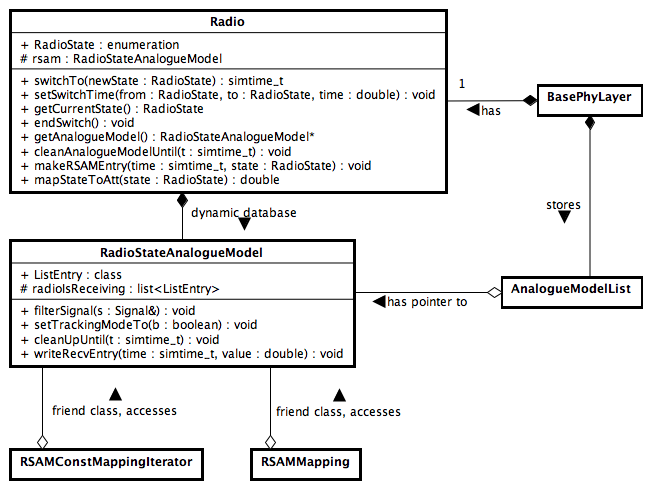
\includegraphics[width = \textwidth]{modelling/Radio_detail.png}
 \caption{The Radio class}
 \label{fig: radio}
\end{figure}

\subsection{AnalogueModel}
%\label{AM and Signal}

%The Signal is designed one-dimensional (power-over-time) by default with a
%specified time point for start and end of the Signal. The owner is able
%to add and request values at a specific time point\req{defsendInfoTXPower}.
%The Method getTimeIterator() returns an appropriate SignalTimeIterator needed
%for applying AnalogueModels to the Signal.

%\begin{quote}
%\emph{NOTE: Anyone who subclasses Signal should make shure to have a properly
%working SignalTimeIterator (subclassed) for it. The SignalTimeIterator should
%always iterate over every time stamp in each dimension. This way simple
%AnalogueModels will be able to filter the Signal independent from its
%dimension.}
%\end{quote}

%Further the Signal is set the packets bitrate over
%time\req{defsendInfoBitrate}, 
%the Move of the Host\req{defsendInfoMove}, the size of the
%packet\req{defsendInfoSize} and the channel dimensions\req{defsendInfoChannel}
%by
%\h{\bp}.
%
%\emph{See also \ref{AirFrame and Signal}.}

The AnalogueModel is at least able to filter the \emph{TX-Power over
time}-Signal.\\

Information how it works on a more complex multi-dimensional Signal are
explained in section \ref{sec:signaldetail}.
 
\begin{figure}[H]
 \centering
 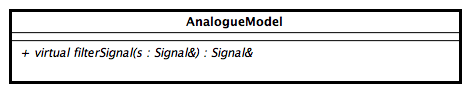
\includegraphics[width = \textwidth]{modelling/AnalogueModel_members.png}
 \caption{analogue model interface}
 \label{fig: analogue model interface}
\end{figure}
%
%The AnalogueModel offers functionality to filter a referenced
%signal\req{defanalogueFilter} in a specified interval\req{defrcvFilterSignals}
%(e.g.
%preamble\req{defrcvFilterPreamble}) or at a single point in time.

%Three basic AnalogueModel classes are foreseen to be plugged into Phy-Layer to
%simulate pathloss\req{defanalogueSimPathloss},
%shadowing\req{defanalogueSimShadowing}
%and fading\req{defanalogueSimFading}.\\
%\h{\bp} is designed to apply an arbitrary number of AnalogueModels to a Signal.

% \begin{figure}[H]
%  \centering
%  \includegraphics[width =
%0.8\textwidth]{modelling/apply_analogue_modells_detail.png}%[width=300pt]
%  \caption{application of analogue models}
%  \label{fig: application analogue models}
% \end{figure}



\subsection{ChannelInfo}

ChannelInfo keeps track of all AirFrames on the channel. It does not
differentiate between \textit{signal} and \textit{noise}. \h{\bp} is able to
add and remove references to certain AirFrames to and from ChannelInfo.\\
ChannelInfo can identify all AirFrames that intersect with a
given time interval and write them to an output-vector.

\begin{figure}[H]
 \centering
 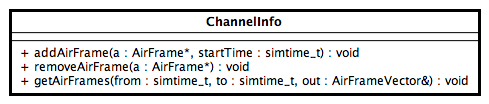
\includegraphics[width = \textwidth]{modelling/ChannelInfo_members.png}
 \caption{channel details}
 \label{fig: channel details}
\end{figure}


\subsection{Decider and DeciderToPhy interface}
\label{decider}

The main task of the Decider is to decide which packets should be handed up to
the MAC layer. To achieve this the \h{\bp} hands every receiving AirFrame
several times to the ``processSignal()``- function of the Decider.

\label{ProcessSignal}
The most common case how a Decider would process AirFrames would be the
following:

\begin{enumerate}
 \item If the Decider gets an AirFrame for the first time, it determines the
time point it can decide if the packet is noise or not and returns this time
point to the \h{\bp}. The time point could be the preamble length, for example.

 \item The next time the Decider gets the packet it would internally decide if
the packet has to be considered noise or not. If the decision is noise the
packet isn't interesting anymore for the Decider. If the packet is classified
as a signal the Decider would return the end of the signal to the \h{\bp}.

 \item When the receiving of the AirFrame is over and the AirFrame wasn't
classified as noise, the Decider would decide if the packet was received
correctly. If the result is positive the Decider has to tell the \h{\bp} to
send the AirFrame together with the DeciderResult to the \h{\bm}.
\end{enumerate}

A second task of the decider is to decide if the channel is busy or idle at a
specific point in time or during a given interval.\\

Since the Decider is responsible to decide if an AirFrame should be
decapsulated and handed up to the MAC layer the Decider needs an interface to
the \h{\bp}.\\

Over the interface the Decider can do the following things:

\begin{itemize}
 \item get the current simulation time
 \item get the list of AirFrames which intersect which a specific interval (to
calculate SNR)
 \item tell the \h{\bp} to hand an AirFrame up to the MAC layer
 \item tell the \h{\bp} to send a control message to the MAC layer
\end{itemize}

Due to the last point the Decider is able to answer a ChannelSenseRequest of the
MAC layer.\\

A Decider that gives a more detailed DeciderResult (e.g. bitwise
errors\req{defdeciderBitwise}) must be subclassed and implemented by the user.

\begin{figure}[H]
 \centering
 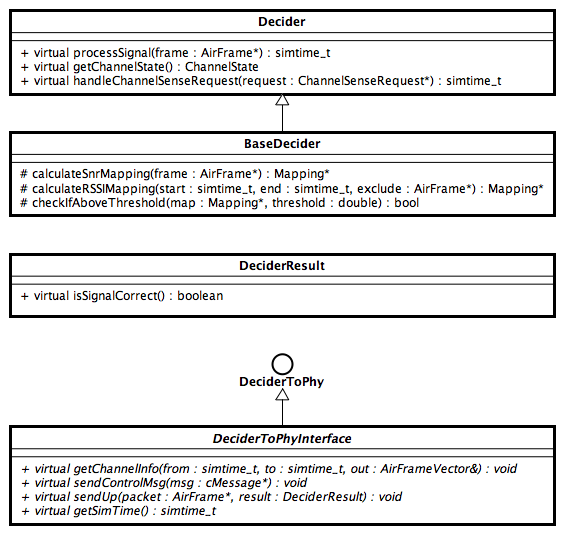
\includegraphics[width = \textwidth]{modelling/DeciderModule_members.png}
 \caption{Decider interface}
 \label{fig: Decider interface}
\end{figure}

\newpage

\subsection{The one-dimensional Signal and AirFrame}
\label{AirFrame and Signal}

AirFrame and Signal both hold information about the packet to send. While the
AirFrame is responsible for the OMNeT related data which is necessary to send
OMNeT messages, the Signal holds the data which is necessary for the simulation
of the transmission process.\\

Here we focus on the basic, one-dimensional (time) Signal that stores entries
for TX Power and attenuation over time\footnote{The time stamps are values
relative to starting time point}. There are fix entries for header and
payload bitrate. These assumptions are considered to cover most cases.
It is possible to obtain a time iterator for this Signal to have access to
entries at specific time points.

Further Signal stores the Move (move pattern of the sending host), the packets
header length, the start time and length of the Signal.\\

\emph{Note: The multi-dimensional Signal is an instance of the same class but
has more functionality. It is described in detail in a separate section.}\\

To be able to control the sending process\req{defsendControl} of an AirFrame
every AirFrame has a unique id and a specific type which specifies if this is a
normal AirFrame or a control-AirFrame. Further it holds an instance of Signal
which represents the physical signal.


\begin{figure}[H]
 \centering
 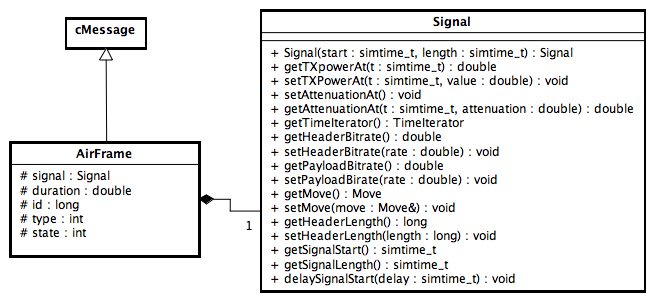
\includegraphics[width = \textwidth]{modelling/AirFrame_members.png}
 \caption{member arrangement in AirFrame and Signal}
 \label{fig:memberAirFrame}
\end{figure}
\newpage

\subsection{receiving a MacPkt}

On reception of a MacPkt from the MAC layer, \h{\bp} checks if:
\begin{enumerate}
	\item the radio is in TX state\req{defsendPreqMode},
	\item it is not already sending a packet\req{defsendPreqSending} 
\end{enumerate} 

If one of these conditions is not fulfilled it will throw an error.\\

The MacToPhyControlInfo object attached to the MacPkt contains the information
needed by \h{\bp} when constructing the AirFrame to send to the channel.
Right now it only contains the Signal initialized by the \h{\bm}.

See \ref{SignalCreation} for how the Signal is created by the \h{\bm}.

\begin{figure}[H]
 \centering
 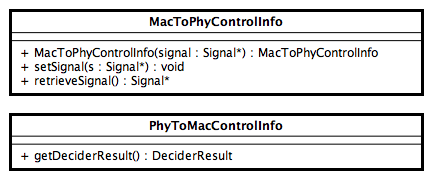
\includegraphics[width = \textwidth]{modelling/MacToPhyCtrlInfo_members.png}
 \caption{MacToPhyControlInfo interface}
 \label{fig: MacToPhyCtrlInfo interface}
\end{figure}


\h{\bp} adds further information to the Signal and is responsible for creating
and initializing the AirFrame and attaching the Signal to it.
For detailed arrangement of information in Signal and AirFrame see \ref{AirFrame
and Signal}.
When the AirFrame is complete and sent, \h{\bp} schedules a TX\_OVER message to
the \h{\bm} (via control-message).

\begin{figure}[H]
 \centering
 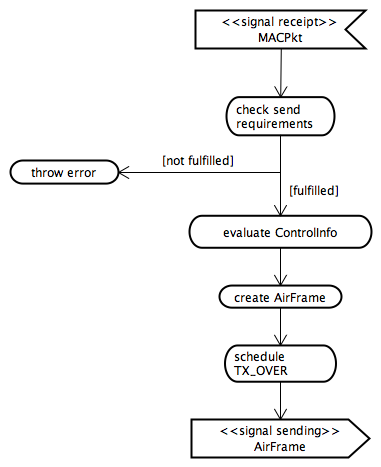
\includegraphics[width = 0.8\textwidth]{modelling/onMACPkt.png}
 \caption{sending process}
 \label{fig: sending process}
\end{figure}
\newpage



\subsection{Receiving and processing an AirFrame}

On arrival of an AirFrame \h{\bp}:
\begin{enumerate}
	
	\item applies AnalogueModels to the corresponding
Signal\req{defrcvSimAttenuation},
	\item receives the AirFrame\req{defrcvSimDuration}.
\end{enumerate}

\begin{figure}[H]
 \centering
 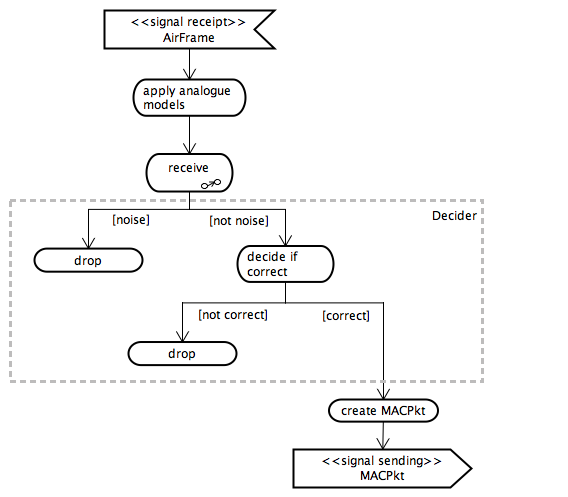
\includegraphics[width = \textwidth]{modelling/onAirFrame.png}
 \caption{receiving process}
 \label{fig: receiving process}
\end{figure}


The receiving process works as follows: In general, time intervals during
reception are simulated by scheduling the AirFrame accordingly.\\

\textbf{stage 0:}\\
An optional propagation delay is simulated by updating the starting time of the
Signal\req{defrcvSimDelay} according to the delay and scheduling the AirFrame to
the reception start point.\\

\textbf{stage 1:}\\
On reception start the Signal is given to the Decider for processing. The
Decider returns a time point it wants to process the Signal again.
This time point has to be before the end of the Signal otherwise an error
is thrown. \\

\textbf{stage 2:}\\
The AirFrame is scheduled arbitrary times for the Decider processing method
until it either returns a negative time point or the time point of the end of
the
Signal. In both cases the state is increased by one before the AirFrame is
scheduled to its end. See \ref{ProcessSignal} for more details on the Deciders
Signal processing. \\

\textbf{stage 3:}\\
Finally reception is over and the AirFrame is completely received in reality.

\emph{Note: The Decider process is responsible for telling the \h{\bp} to send
a MacPkt to the \h{\bm}.}

\begin{figure}[H]
 \centering
 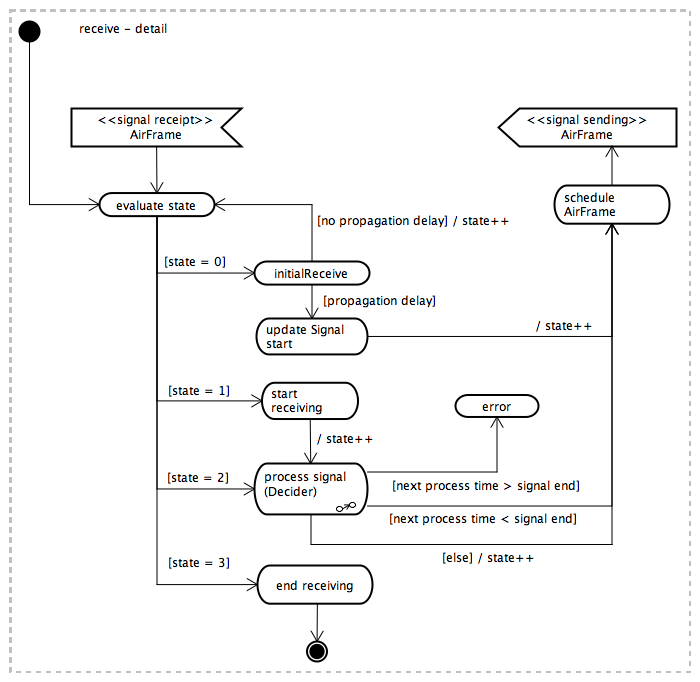
\includegraphics[width = \textwidth]{modelling/receive_detail.png}
 \caption{receive detail}
 \label{fig: receive detail}
\end{figure}


% The receiving process is modelled internally by a state machine that schedules
%the AirFrame that is received (since we have a pointer to it from the
%beginning) everytime a delay/time interval shall be simulated. That saves us
%the creation of additional self-messages.




%When the preamble of a packet is completely received, \h{\bp} constructs a
%SNInfo for the preamble, applies the AnalogueModels to it and passes it to the
%Decider to find out whether this packet is considered noise.

%\begin{figure}[H]
% \centering
% \includegraphics[width = 0.2\textwidth]{modelling/end_preamble_detail.png}
% \caption{end preamble detail}
% \label{fig: end preamble detail}
%\end{figure}

%In case a received packet is not \textit{noise} it is processed, i.e. \h{\bp}
%creates the corresponding SNInfo for the packet, applies AnalogueModels to it
%and passes the result to the Decider to check whether the packet was received
%correctly. If so, a MacPkt is created and handed up to
%Phy-Layer\req{defrcvPassToMAC}.


\subsection{the .ned-file}

The .ned-file of the \h{\bp} has the following parameters:

\begin{itemize}
\item usePropagationDelay as \textit{boolean}\req{defconfDelay}
\item analogueModels as
\textit{XML}\req{defconfAnalogue}\req{defconfAnalogueParam}
\item decider as \textit{XML}\req{defconfDecider}\req{defconfDeciderParam}
\item thermalNoise as \textit{numeric const}\req{defconfNoise}
\item sensitivity as \textit{numeric const}\req{defconfSens}
\item maximal TX power as \textit{numeric const}\req{defconfMaxTXPower}
\item switchTimeRX as \textit{numeric const}\req{defconfSwitchingTimes}
\item switchTimeTX as \textit{numeric const}\req{defconfSwitchingTimes}
\item switchTimeSleep as as \textit{numeric const}\req{defconfSwitchingTimes}
\end{itemize}

The parameters "analogueModels" and "decider" store which AnalogueModels and
which Decider are to be used, together with their parameters in XML format. The
exact format still has to be declared!

%\subsection{provide status information to MAC}

%Passively provided information\req{defprovpassive}: \h{\bm} is equipped with a
%reference to \h{\bp} in order to obtain information
%about channelstate\req{defchannelstate} and current radio
%state\req{defcurrentmode}
%by
%simple method calls. \\
%Actively provided information\req{defprovactive}: A cMessage of the kind
%TX\_OVER
%is sent to MAC layer when a sending transmission is over\req{deftxover},
%\saf{sending process}.



%\subsection{send packets}

%Since \h{\bm} has a reference to \h{\bp} it can obtain information about the
%state the radio is is currently in\req{defsendPreqMode}, it is not already
%sending
%to the channel on its own\req{defsendPreqSending} and the channel is
%idle\req{defsendPreqIdle} via method calls, \saf{BasePhyLayer interface}.

%The class MacToPhyControlInfo is designed as the container for control
%info\req{defpacketFromMac} the MAC layer
%wants to attach to the packet given down to Phy-Layer for sending.
%The packet itself is handed down as a MacPkt via OMNeT-channel. 



\subsection{signal details}
\label{sec:signaldetail}

For a complex signal transmission power, bitrate and attenuation of a Signal
can be mathematical mappings from space, frequency and time to double. So
we decided to store each of them by the ``Mapping``-interface which is able to
represent a mathematical mapping from an arbitary domain (time + $\mathbb{R}^n$)
to a double ($\mathbb{R}$) value.

\begin{figure}[H]
 \centering
 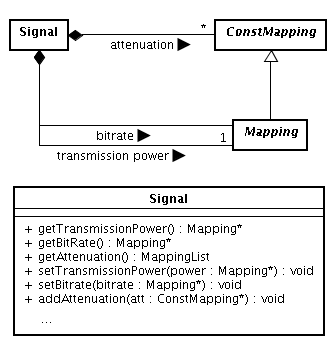
\includegraphics[width = 0.6\textwidth]{SignalDetail/signal_members.png}
 \caption{signal members (TX-power, bitrate and attenuation)}
 \label{fig:signal members detail}
\end{figure}

ConstMapping represents a mathematical mapping which can not be changed
arbitary, see section \ref{mapping detail} for details.

So transmission power, bitrate and attenuation are each seperate Mappings. To
get the filtered (attenuated) transmission power its Mapping is multiplied with
every attenuation Mapping.
\newpage

\subsubsection{Mapping overwiev}

Since Mappping has to be able to map from an arbitary domain (with arbitary
dimenensions) to a double value we need some structures to represent a
dimension, a domain and the arguments for a mapping in a specific domain.

This leads to the following structure.

\begin{figure}[H]
 \centering
 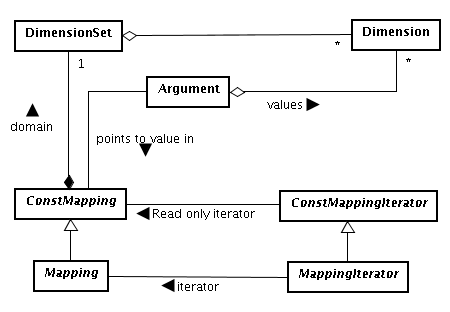
\includegraphics[width = 0.82\textwidth]{SignalDetail/mapping_detail.png}
 \caption{mapping details}
 \label{fig:mapping detail}
\end{figure}

\begin{figure}[H]
 \centering
 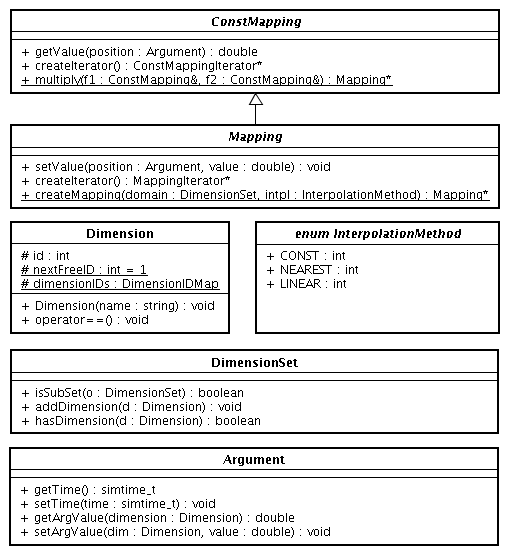
\includegraphics[width = 0.9\textwidth]{SignalDetail/mapping_members.png}
 \caption{mapping members}
 \label{fig:mapping members}
\end{figure}

Every instance of DimensionSet has at least the time as Dimension.
\newline

An instance of the Mapping interface has to provide random read and write access
per setValue() and getValue() method. This means if you call setValue() with an
valid Argument and the new value any following call of getValue() with the same
Argument has to return the new value.
\newline

%TODO: interpolation

Since the attenuation mappings does only need random read access but no write
access there is the ConstMapping-interface which basically is a Mapping without
the setValue()-method (or more precisely, Mapping is a ConstMapping with a
setValue()-method). This way we are able to implement ConstMappings which
represent a simple (probably parameterised) mathematical function like a sinus
curve.
\newline

The Mapping interface provides a multiply functions which is able to multiply
instances of Mappings with each other. This method is used by the decider to
get the attenuated transmission power.
\newline

To create an instance of a class which implements the Mapping interface one can
use the static createMapping()-method which creates a Mapping with the passed
DimensionSet as domain. If the DimensionSet parameter is ommited it creates an
Mapping with only time as domain. See section \ref{mapping detail} for details
on the returned Mapping implementation.

\subsubsection{iterating a Mapping}

The MappingIterator-interface provides an uniform way to iterate independent
from the underlying Mapping implementation.

\begin{figure}[H]
 \centering
 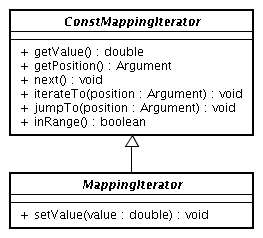
\includegraphics[width = 0.5\textwidth]
	{SignalDetail/mapping_iterator_member.png}
 \caption{mapping iterator details}
 \label{fig:mapping iterator detail}
\end{figure}

The next()-method iterates to the next position in the mapping, where this next
position actually is depends on the implementation of the Mapping. For
continous Mappings like the sinus curve this probably whouldn't be a particular
meaningful value. In fact this method is rather meant to be used for
implementations which use a number of key entries between which is interpolated.
But independent of the implementation of the underlying Mapping every iterator
has
to make sure that the Argument value of the position after the call of next is
compared greater than the Argument of the position before. This is possible
because Arguments can be sorted by the unique ids of their dimensions and the
the according values of the Argument.
\newline

While the jumpTo()-method is able to move the Iterator to an arbitary (but
valid) specified position the position passed to the iterateTo()-method has to
be greater or equal to the current position of the iterator. Furthermore the
iterateTo()-method assumes that the passed new position is near the current
position of the iterator, if this prerequirement is met iterateTo() is faster
than the jumpTo()-method.
\newline

Similar to ConstMapping the ConstMappingIterator is just a MappingIterator
whithout the setValue()-method.

\subsubsection{Mapping detail}
\label{mapping detail}

The type of the Mapping implementation returned by the createMapping()-method
of the Mapping interface depends on the passed DimensionSet parameter. If the
parameter is omitted or the DimensionSet defines only time as dimension the
returned Mapping is of type TimedMapping, otherwise it is of type
MultiDimMapping.

\subsubsection{TimedMapping}

The TimedMapping works only for Mappings with only time as domain. The mapping
is implemented by a std::map which takes the time as key. At every call of
setValue() the value is stored with the passed time as key in the map.
A call to getValue() returns the previously stored value in the map if
available, if no value is stored at this position it interpolates between the
nearest entries in the map to calculate the value at the queried position. 
\newline
%TODO: interpolation method

The MappingIterator for the TimedMapping makes use of the iterator of the
std::map. Since a MappingIterator has to be able to iterate to any
position inside the range of the domain of the Mapping but the map-iterator can
only point to actual values inside the map the MappingIterator also stores the
actual position together with the map-iterator. 

Here is a short description what the methods of the MappingIterator of a
TimedMapping do:

\begin{description}
 \item getValue() uses the map-iterator and the stored actual position
to calculate the actual value (per interpolation).
 \item next() simply increases the map-iterator by one to the next
entry in the map. 
 \item jumpTo() sets the map-iterator to the entry next to
the position passed as parameter and stores the passed position as actual
position.
 \item iterateTo() increases the map-iterator until it points to an entry
near the position passed as parameter and stores the passed position as actual
position.
\end{description}

\subsubsection{MultiDimMapping}

The MultiDimMapping is able to represent any Mapping with at least one
other Dimension besides the time as domain. The multiple dimensions are realized
by a map of Mappings. Every MultiDimMapping has a std::map from double to
pointers to Mapping (\verb std::map<double, \verb Mapping*> ).
So a simple two-dimensional Mapping (time and channel for example) whould be a
MultiDimMap which map stores for every channel a sub-mapping. Every
sub-mapping whould be of type TimedMapping and represent the gradient over time
for the according channel.

The following figure visualizes the general structure of a multi-dimensional
mapping with MultiDimMapping.

\begin{figure}[H]
 \centering
 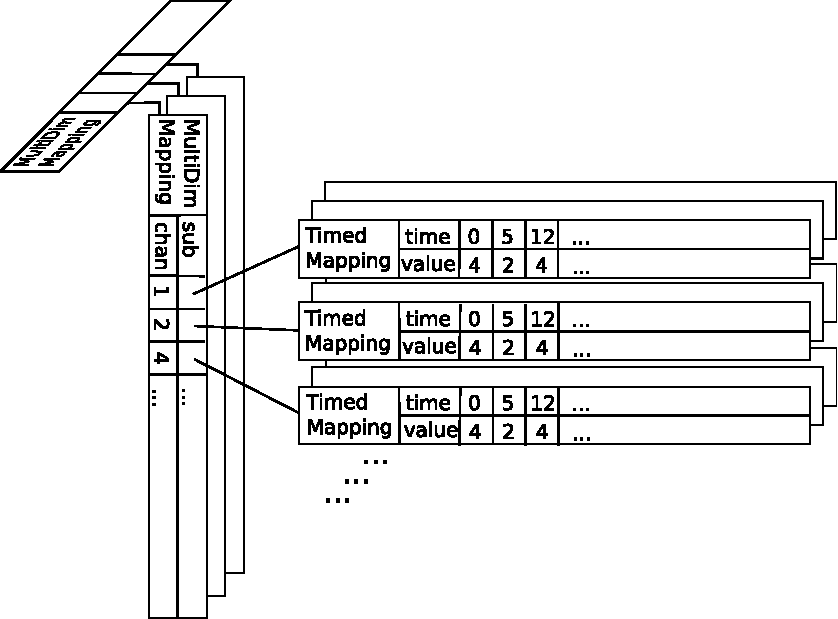
\includegraphics[width = 0.9\textwidth]{SignalDetail/mapping_scheme.pdf}
 \caption{multi dimensional signals}
 \label{fig:mappingscheme}
\end{figure}

So every dimension of the domain is represented by a layer of instances of
MultiDimMapping (respectively TimedMapping for the last dimension - which is
always the time).
The order of the layers is determined by the Dimensions and therefor is the
same for every MultiDimMapping instance.
\newline

Like the TimedMapping a MultiDimMapping can not store a value for every
possible position in the domain of the Mapping. Therefore a call to getValue()
whould determine the sub-Mappings near the position of the passed
Argument-parameter and pass the Argument-parameter to the getValue()-Methods of
the near sub-Mappings, then it interpolates between the returned values. Thus
getValue() is realized by recursive calls of getValue() and interpolation
between their return-values.
\newline 

Iteration is implemented the same way, meaning recursively. Like the
TimedMappingIterator the MultiDimMappingIterator stores the current position
(as a member of type Argument) together with a map-iterator pointing to the
entry inside the map of sub-Mappings near the current position.
Besides that it also stores an MappingIterator for the sub-Mapping at the
current position. This is necessary because the mapping has to be able to
iterate recursively over the sub-mappings.
\newline
%TODO:interpolation

Here is a short description what the methods of the MappingIterator of a
MultiDimMapping do:

\begin{description}
 \item getValue() calls recursively the getValue() method of the
MappingIterator of the sub-mapping at the current position.
 \item next() calls hasNext() at the MappingIterator of the
sub-mapping, if it returns true its next() method is called, otherwise the
map-iterator for the current sub-mapping is increased by one to the next
entry and a MappingIterator for the new position is created. Thereby it is
assured that the entries in the whole Mapping are iterated in the correct order.
\item jumpTo() and iterateTo() work more ore less like the methods for the
TimedMappingIterator.
\end{description}
%\section{Appendix}

%\begin{figure}[h]
% \centering
% 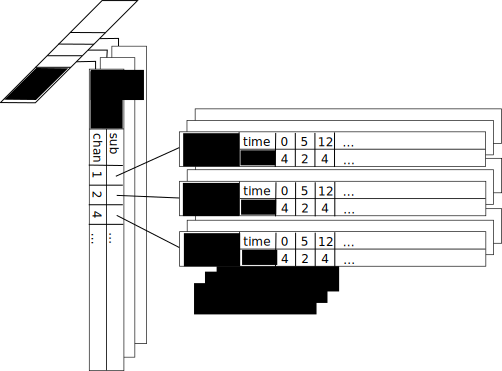
\includegraphics[width=400pt]{signal/signal.pdf}
% \caption{class graph}
% \label{fig: signal abstract}
%\end{figure}

%\begin{figure}[h]
% \centering
% 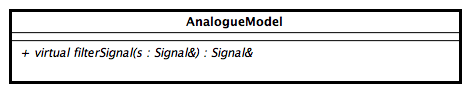
\includegraphics[width=340pt]{modelling/AnalogueModel_members.png}
% \caption{analogue model interface}
% \label{fig: analogue model interface}
%\end{figure}

%\begin{figure}[h]
% \centering
% 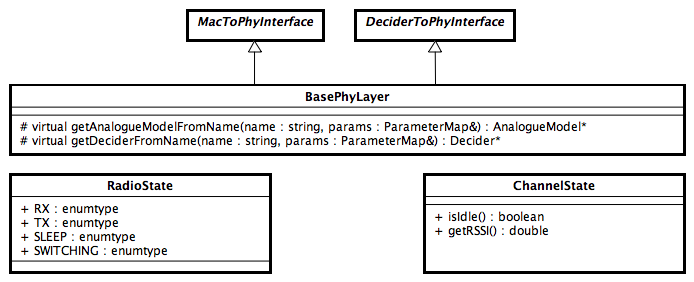
\includegraphics[width=340pt]{modelling/BasePhyLayer_members.png}
% \caption{BasePhyLayer interface}
% \label{fig: BasePhyLayer interface}
%\end{figure}

%\begin{figure}[h]
% \centering
% \includegraphics[width=340pt]{modelling/DemodulationModule_members.png}
% \caption{Demodulator interface}
% \label{fig: Demodulator interface}
%\end{figure}

%\begin{figure}[h]
% \centering
% 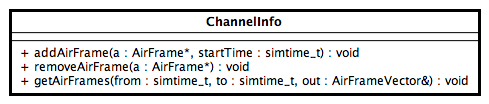
\includegraphics[width=340pt]{modelling/ChannelInfo_members.png}
% \caption{channel details}
% \label{fig: channel details}
%\end{figure}

%\begin{figure}[h]
% \centering
% 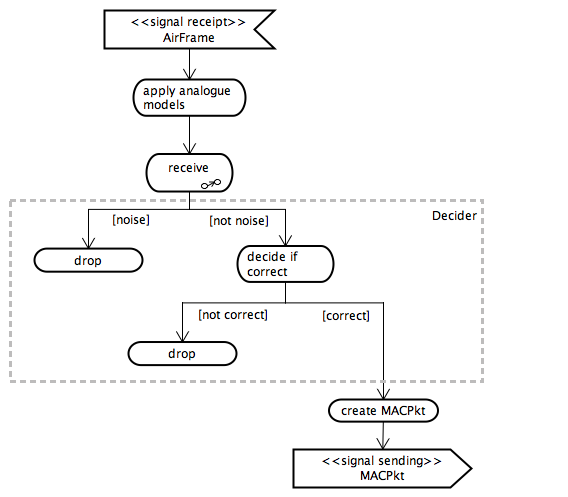
\includegraphics[width=340pt]{modelling/onAirFrame.png}
% \caption{receiving process}
% \label{fig: receiving process}
%\end{figure}

%\begin{figure}[h]
% \centering
% 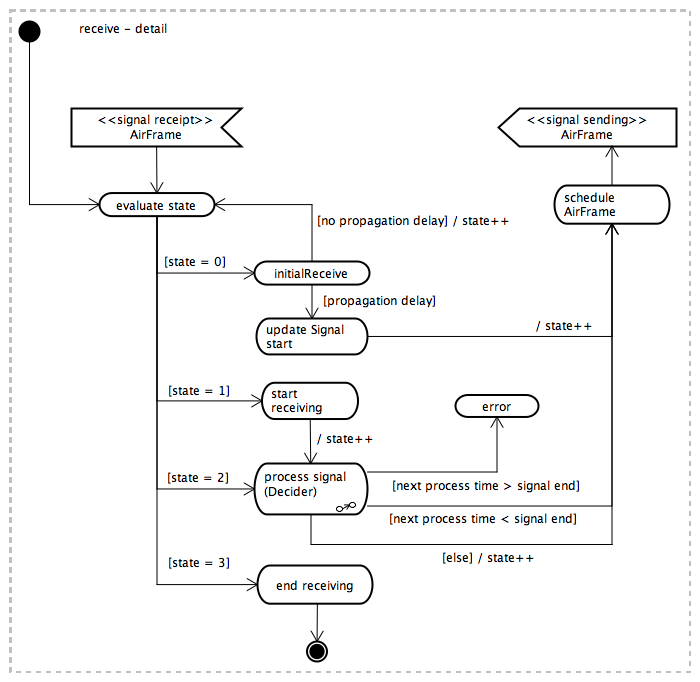
\includegraphics[width=340pt]{modelling/receive_detail.png}
% \caption{receive detail}
% \label{fig: receive detail}
%\end{figure}

%\begin{figure}[h]
% \centering
% 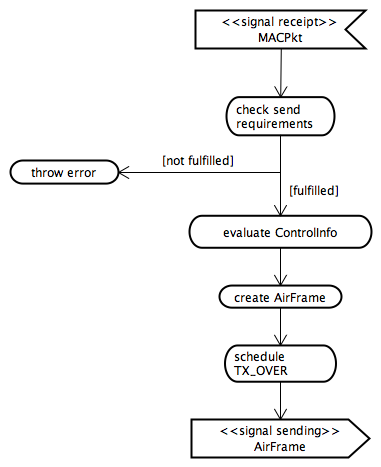
\includegraphics[width=300pt]{modelling/onMACPkt.png}
% \caption{sending process}
% \label{fig: sending process}
%\end{figure}


\end{document}
